In this study, we are focusing on providing an overview of the
research on gamification applied to education [5][16]. Furthermore,
it is worth mentioning that this mapping study is part of an ongoing
project whose purpose is to investigate gamification and Computer
Supported Collaborative Learning (CSCL). Thus, as a secondary
objective of this systematic mapping, we also aim to identify the
existence of initiatives that use gamification in CSCL
environments. 

\todo[inline]{FAZER O UPDATE E ESCREVER AQUI NOVOS  DADOS - CITAR O ONLINE QUANTO PRECISO}

%---------------------------------------------
% The Systematic Mapping Process
%---------------------------------------------
\section{The Systematic Mapping Process}

We carried out our study by following the process described by
[26]. According to them, systematic mappings are a fivefold
process: (i) definition of research questions, (ii) performing the
search for relevant primary studies, (iii) screening of papers, (iv)
keywording of abstracts, and (v) data extraction and mapping.
Research questions have to incorporate the study purpose. Thus,
since we set out to ascertain what aspect of gamification applied to
education has been most investigated by researchers, our three
research questions (RQs) reflect this purpose as the following:
RQ1: In what educational contexts and levels has gamification been
most investigated?
RQ2: What types of studies have been most investigated in
gamification and education?
RQ3: What gamification approaches have been most investigated
in the field of computer-supported collaborative learning (CSCL)?
Based on these questions we defined inclusion and exclusion
criteria. These criteria are important to identify relevant primary
studies that answer the RQs. We devised the following inclusion
criteria:
 If several papers reported the same study, only the most recent
paper was selected;
 If the paper describes more than one study, each study was
assessed individually.
And the following exclusion criteria:
 Papers that do not present studies relating to education;
 Papers in languages other than English;
 Technical reports and documents that are available in the form of
summaries or presentations (gray literature) and secondary
studies (i.e., systematic literature reviews and mapping studies).
At first, we ran some searches using a combination of candidate
keywords. These trial searches combined the keyword gamification
with some synonyms related to education and learning. Due to the
217
small number of papers returned from the resulting strings, we
decided that only the keyword gamification should be used.
This decision allowed us to analyze a greater number of papers,
lowering the odds of leaving relevant studies out of our final set.
Using gamification as keyword, we performed searches on
electronic databases that are known to cover relevant scientific
journals and articles from a wide variety of domains such as
Computer Science, Education and Educational Research, Science,
Engineering, Medicine and Psychology. Initially, we retrieved 357
primary papers. However, only 48 candidate papers were obtained
after applying the inclusion and exclusion criteria based upon title
and abstract. Finally, after going over introductions and
conclusions, we ended up with a final set of 26 primary papers as
shown in Table~\ref{tab:distribution_of_primary_studies}. The complete list of these papers can be obtained
at: http://goo.gl/KUH1m. 


\begin{table}[]
\centering
\caption{Distribution of primary studies by electronic database }
\label{tab:distribution_of_primary_studies}
\begin{tabular}{|l|l|}
\hline
\textbf{Database}         & \textbf{Quantity} \\ \hline
ACM Digital Library       & 144               \\ \hline
Elsevier (Science Direct) & 32                \\ \hline
IEEE Xplore               & 31                \\ \hline
Scopus                    & 95                \\ \hline
Springer                  & 55                \\ \hline
Total                     & 357               \\ \hline
Candidates                & 48                \\ \hline
Final Selection           & 26                \\ \hline
\end{tabular}
\end{table}

We read all 26 papers in full and applied a keywording strategy to
devise our classification scheme and categories for the selected
primary studies. At first, abstracts were read in order to find
keywords and concepts that reflect the contribution of the studies.
After reading the papers, the keywords and concepts were
combined to synthesize the nature of the selected contributions.
Finally, the final set of keywords was used to define representative
categories. As a result, the following categories were defined to
better understand and classify the primary studies:
Mastering Skills: in this category we included all studies that
propose the use of gamified systems as a means to improve
students' ability to perform activities considered complex or
repetitive.
Challenging: this category includes studies whose authors claim
that gamified systems that implement challenging activities can
contribute to the improvement of learning.
Guidelines: this category includes studies whose authors consider
how gamification can be applied in educational settings. These
studies, however, do not provide empirical evidence that backs up
the authors' claims. Usually, these papers are built on results of
other researchers.
Engagement: studies in this category describe approaches or
strategies to arouse and maintain students' interest in learning a
given subject.
Improving Learning: this category includes studies that propose
gamified solutions to enhance the way students learn, maximizing
the results of the learning process.
Behavioral change: this category includes studies that propose
using gamified systems in order to foster behavioral changes in
students.
Socialization: studies in this category discuss that learning can take
place under more favorable conditions when supported by gamified
social tools.

%---------------------------------------------
% Discussion - Analysis
%---------------------------------------------
\section{Discussion} 

In this section we analyze the results of our mapping study. The
purpose of this section is to give an overview of how gamification
has been used to support education. The information drawn from
the selected primary studies is also used to answer our mapping
study's research questions.
To answer our first question (i.e., in what educational contexts and
levels have gamification been most investigated?) we analyzed the
primary studies and categorized them according to the target
audience (Table~\ref{tab:target_audience}). In Table~\ref{tab:target_audience} we can observe that most primary
studies present gamification approaches tailored towards
supporting higher education students (46\%). Thus, we can conclude
that the answer to RQ1 is that gamification has been mostly applied
in approaches to teaching students in higher education. On the other
hand, among the selected primary studies, elementary education is
the stage of education drawing less attention: only two primary
studies, which accounts for only 8\% of the selected studies, discuss
gamification-based approaches for teaching elementary students.
As for the other studies, six primary studies (23\%) describe the
benefits and shortcomings of gamification-based models and
educational strategies. These six studies, however, fail to position
themselves in “the big picture”. In other words, the authors do not
mention in which educational level (e.g., elementary or higher
education) their approaches should be incorporated so that one can
best grasp the benefits of such approaches in particular educational
contexts. In fact, none of these six primary studies mention whether
or not gamification can be applied in educational level curricula.
 
\begin{table}[]
\centering
\caption{Primary studies categorized according to target
audience or subject matter}
\label{tab:target_audience}
\begin{tabular}{|l|r|r|}
\hline
\textbf{Target audience}   & \multicolumn{1}{l|}{\textbf{Number}} & \multicolumn{1}{l|}{\textbf{Frequency(\%)}} \\ \hline
Higher Education           & 12                                   & 46.15\%                                     \\ \hline
Non-specific context/level & 6                                    & 23.08\%                                     \\ \hline
Training and Tutorials     & 3                                    & 11.54\%                                     \\ \hline
Languages                  & 2                                    & 7.69\%                                      \\ \hline
Elementary Education       & 2                                    & 7.69\%                                      \\ \hline
Lifelong Education         & 1                                    & 3.85\%                                      \\ \hline
\end{tabular}
\end{table}

The other studies either discuss or propose using gamification
models with the following purposes: training and tutorials (12\%),
teaching and learning languages (8\%), and supporting students
tackling lifelong education \footnotetext{Further Education in Great Britain.}
 projects (1\%). It is worth mentioning that none of the selected studies described gamification approaches whose target audience is preschool, high school, or disabled
students.
There has been a recent growing interest in research on developing
e-learning environments that are equipped with gamification
elements and techniques. Table 3 presents the primary studies
clustered by date of publication. Although the first publications
appeared only in 2011, the number of studies on gamification more
than doubled from 2011 to 2012. As for 2013, taking into account
only January and February, the months during which this study was
carried out, three studies had already been published. It is important
to note that several articles related to gamification have been
published before 2011. Nevertheless, most of them were not related
to education and none of them met the inclusion/exclusion criteria
defined in our study. This result reveals that gamification applied
to education is becoming a new research trend with room for new
findings and improvements. To proper understand the impact
(positive or negative) and implications of using gamification in
educational contexts there is a need for more research and empirical
data. 

Table 3. Overview of the distribution of the selected studies
throughout the years

Most primary studies were published by either ACM DL (ACM
Digital Library) or Springer, as shown in Table 4. The electronic
databases, Elsevier (ScienceDirect) and IEEE (IEEE Xplore) had
five and three selected studies, respectively. We also searched
through Scopus, however, given that it was the last electronic
database to be examined, most primary studies it indexes had
already been selected from one of the aforementioned electronic
databases. Four studies were selected from Scopus; these studies
had not been returned by the other electronic databases. 

Table 4. Distribution of the primary studies according to
electronic database

By analyzing where the primary studies were published, we found
that there is no specific venue whose purpose is to bring together
research on gamification applied to education. The most notable
publication forums according to the number of selected primary
studies are the following: the American Society for Engineering
Education Annual Conference (ASEE) (two studies were published
in 2012) and the ACM eLearn Magazine (two studies as well).
Furthermore, three primary studies were book chapters from the
book Serious Games and Edutainment Applications published in
2011 by Springer [22].
Regarding the publication types, we have selected studies that have
been published in journals, magazines, conferences, workshops, symposia, and books. 

Table 5 gives an overview of the primary studies distributed according to publication type. As shown in Table 5, most selected studies are conference publications. Journal
publications are the second most common publication type. It is worth mentioning that most of these journals have a multidisciplinary scope. 

Table 5. Primary studies organized by publication type 

Primary studies frequently use the term “motivation” to justify the
research in question or the main reason behind investigating
gamification. Nevertheless, after an in-depth analysis of these
studies, we found that several objectives fall under the term
“motivation”. Thus, we were able to identify seven different
objectives: (i) Mastering skills: improving certain abilities of the
students; (ii) Challenging: proposing challenges that give extra
meaning to the learning process; (iii) Engagement: engaging
students in learning activities that are more interesting and easier to
follow; (iv) Improving learning: maximizing the acquisition of
knowledge; (v) Behavioral change: fostering changes of behavior
by rewarding adequate actions and penalizing unsatisfactory ones;
(vi) Socialization: allowing for both socialization mechanisms and
group learning; and (vii) Guidelines: discussing the benefits of
gamification as a means to motivate students and deal with some of
the learning process problems. Our results demonstrate that there
are some overlaps between these seven classification categories.
Apart from identifying the objectives of the primary studies, it is
also important to characterize the type of research that was carried
out and reported in these studies. Towards this end, we applied the
classification proposed in [26]. Such a classification comprises the
following research types.
Validation Research, studies that fall into this category describe a
novel technique, approach, or strategy that has not been
implemented in practice, but whose effectiveness has been
evaluated to some degree through laboratory studies.
Evaluation Research, this category contains studies that
empirically evaluate a technique, approach, or strategy in practice
or real settings.
Position Papers, these studies report the authors' point of view.
Research in this category does not contain evidence that backs up
the authors' opinion.
Philosophical Papers, studies in this category are similar to
position papers, however, they shed light on new ways through
which educational approaches can benefit from gamification.
Solution Proposals, studies that describe a solution technique,
approach, or strategy and argue for its usefulness, such a solution
is either novel or extends an existing approach; studies in this
category usually present examples and good line of argumentation
(but not strong empirical data). 
Experience papers, these studies are concerned with reporting the
author's experience during the implantation of a new approach.
Rather than plotting frequency tables to illustrate the distribution of
the studies according to research type and objectives, we decided
to generate a bubble plot (Figure 2), but the primary studies
summarized in Figure 2 are also shown in Table 6. The resulting
bubble plot is intended to be seen as a map of research on
gamification used in conjunction with education. A bubble plot has
two x-y scatter plots containing bubbles in category intersections.
The size of these bubbles is determined by the amount of primary
studies that have been classified in the pair of categories in
question.
Such a visual summary gives an overview that enables researchers
to pinpoint categories that have been drawing most attention as well
as the ones that have not been much investigated. Therefore, by
analyzing such a map it is possible to identify gaps and
opportunities for future research. The bubble plot generated from
our selected studies is shown in Figure~\ref{fig:bubblemap_gamification}.
By analyzing Figure 2, we can identify that the research objective
of most studies is to evaluate (Evaluation) the engagement
(Engage) of the students through gamification (13 studies). It is also
possible to identify that there are no studies on Experience or
Validation, which answers RQ2 (What types of studies have been
most investigated in gamification and education?). This indicates
there is a lack of validation research that helps to propose novel
techniques/methods and test them in well-thought-out controlled
laboratory experiments. Similarly, it is necessary for more research
to be done with the help of end users, i.e. teachers, to report
personal experiences regarding the application and implications of
using gamification in learning environments. 

\begin{figure}[h!]
\caption{Map containing the distribution of gamification research by study type (x axis) and research objectives (y axis) }
\centering
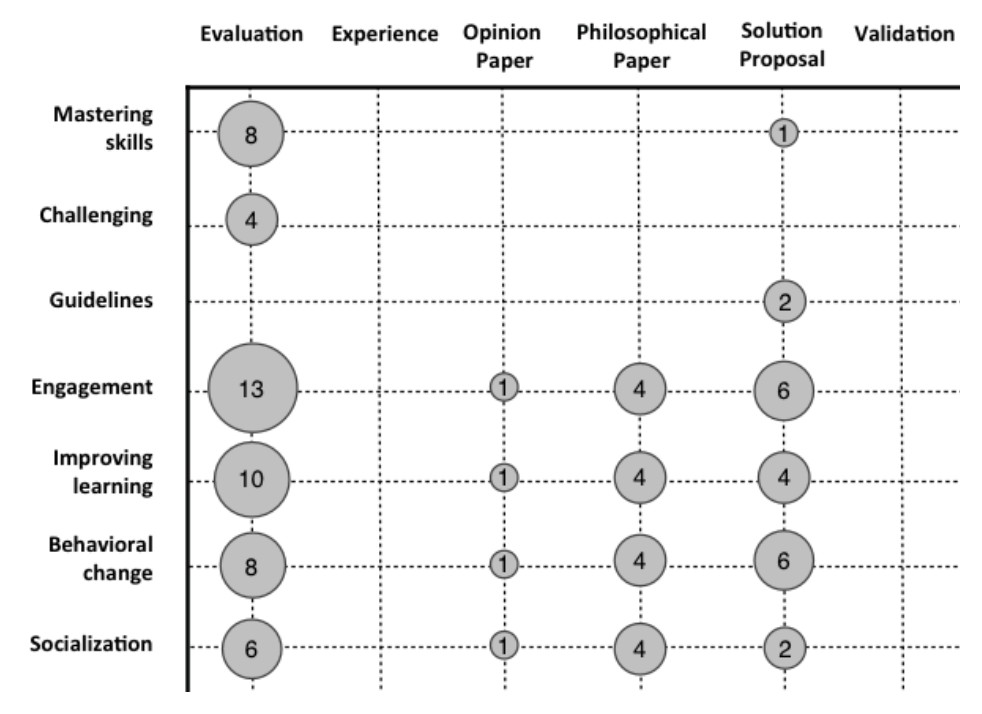
\includegraphics[width=.9\textwidth]{bubblemap_gamification}
\end{figure}

Table 6 also synthesizes the frequency of primary studies according
to research objective. The numbers in parenthesis represent the
number of papers in the category, while the numbers in square
brackets are the papers’ references. 24 of the 26 studies have
Engagement among students as their main objective. Only two
studies do not directly approach such an objective, discussing
motivation in a higher abstraction level. Contributing to further
improvement in how students socialize is mentioned by 13 studies
(Socialization). Nevertheless, only eight primary studies report
practical solutions to achieving such an objective, four encourage group activities, and one highlights the importance of this sort of
activity.

\textbf{Table 6. Distribution of gamification research by study type and research objectives}

A Venn diagram was drawn to clarify the distribution of the
overlapping studies (Figure 3). For simplicity’s sake, we decided to
include only four categories in the diagram. As shown in the
diagram, 9 papers overlap 4 research objectives. Some studies
encompass only two or three research objectives: (i) engagement
and behavioral change; (ii) socialization and engagement; and (iii)
improving learning, behavioral change, and engagement. This
suggests that motivating students is not a straightforward task that
can be accomplished by employing only one strategy. However, the
amount of studies that employ the four main research objectives
indicates that researchers have been striving to come up with more
sound solutions to motivate students.
Only one study mentions that computer-supported collaborative
learning (CSCL) is suited to develop applications that help students
to socialize and organize themselves in groups. However, this study
does not cover how to undertake the integration of computer-supported
collaborative learning, gamification, and educational
approaches. Therefore, the answer to RQ3 (What gamification
approaches have been most investigated in the field of CSCL?) is
that there is a lack of approaches that combine gamification and
computer-supported collaborative learning. 

\textbf{Figure 3. Overview of the four categories with the highest
number of papers and the overlap among them }

%---------------------------------------------
% Threats to Validity
%---------------------------------------------
\section{Threats to Validity}

In order to ensure an unbiased selection process, the RQs, inclusion
criteria, and exclusion criteria were established before the
conduction of the systematic mapping. Furthermore, the selection
process was carried out in an independent fashion by each involved
author. To mitigate any selection bias and improve validity, the
inclusion or exclusion of controversial studies was jointly decided.
Nevertheless, we cannot rule out threats from a quality assessment
perspective because during the selection process no scores were
assigned to studies.
Another threat to validity consists of whether we selected all
relevant studies in the area. Although such a threat cannot be ruled
out, we tried to mitigate it by taking into account several important
search engines. Therefore, we surmise that these search engines are
prone to contain the majority of the relevant studies. In the future,
we intend to update this scoping study by taking into account more
search engines. The coherency of our classification scheme also
represents a threat to the validity of this mapping study. As pointed
out by [27], one of the problems of mappings studies is how to
determine the proper way to categorize the resulting studies. 

%---------------------------------------------
% Concluding Remarks
%---------------------------------------------
\section{Concluding Remarks of the Systematic Mapping}

The main purpose of our mapping study is to provide an overview
of what has been investigated in the context of gamification applied
to education. To fulfill our goal, we followed a systematic
methodology, i.e., systematic mapping. We defined three research
questions to be answered by our mapping. RQ1: In what
educational contexts and levels has gamification been most
investigated? RQ2: What types of studies have been most
investigated in gamification and education? RQ3: What
gamification approaches have been most investigated in the field of
CSCL?
According to our results, most studies were published in
conferences and have focused on Higher Education (RQ1 – see
Table 2) to foster the engagement of students through learning
activities that build on gamification concepts (RQ2 – see Table 6).
We also identified that there is a lack of approaches that combine
gamification and CSCL (RQ3).
The novelty of this research is that, to the best of our
knowledge, this is the first systematic mapping covering research
into gamification applied to education. Another contribution of this
research is the map (Figure 2) we have created. By analyzing such
a map it is possible to identify in which way gamification has been
explored in educational contexts; thereby determining research
gaps and future research opportunities. 
